% PyG File Structure Diagram
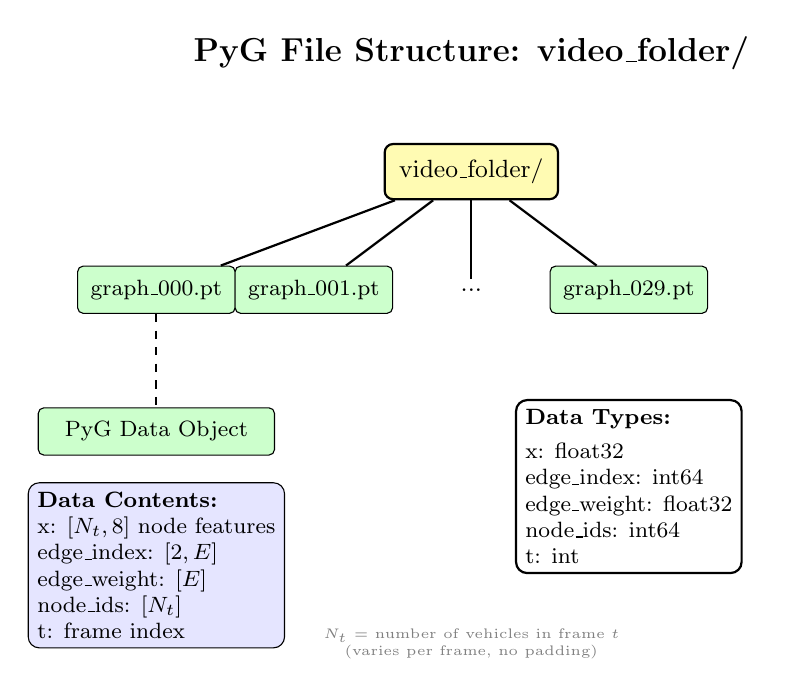
\begin{tikzpicture}[
    folder/.style={
        rectangle,
        rounded corners=3pt,
        draw=black,
        thick,
        fill=yellow!30,
        font=\small,
        minimum height=0.7cm,
        minimum width=2.2cm,
        align=center
    },
    file/.style={
        rectangle,
        rounded corners=2pt,
        draw=black,
        fill=green!20,
        font=\footnotesize,
        minimum height=0.6cm,
        minimum width=2cm,
        align=center
    },
    arrow/.style={draw, thick, -}
]

% Title
\node[font=\bfseries\large] at (4, 3) {PyG File Structure: video\_folder/};

% Root
\node[folder] (root) at (4, 1.5) {video\_folder/};

% Graph files
\node[file] (g0) at (0, 0) {graph\_000.pt};
\node[file] (g1) at (2, 0) {graph\_001.pt};
\node[font=\small] (dots) at (4, 0) {...};
\node[file] (g29) at (6, 0) {graph\_029.pt};

% Connect root to files
\draw[arrow] (root) -- (g0);
\draw[arrow] (root) -- (g1);
\draw[arrow] (root) -- (dots);
\draw[arrow] (root) -- (g29);

% Expand one graph file
\node[file, minimum width=3cm] (data) at (0, -1.8) {PyG Data Object};

\draw[arrow, dashed] (g0) -- (data);

% Data object contents
\node[font=\footnotesize, align=left, fill=blue!10, draw, rounded corners] at (0, -3.5) {
    \textbf{Data Contents:}\\
    x: $[N_t, 8]$ node features\\
    edge\_index: $[2, E]$\\
    edge\_weight: $[E]$\\
    node\_ids: $[N_t]$\\
    t: frame index
};

% Data type annotations box
\node[font=\footnotesize, align=left, fill=white, draw, rounded corners, thick] at (6, -2.5) {
    \textbf{Data Types:}\\[0.1cm]
    x: float32\\
    edge\_index: int64\\
    edge\_weight: float32\\
    node\_ids: int64\\
    t: int
};

% Note about dynamic size
\node[font=\tiny, gray, align=center] at (4, -4.5) {$N_t$ = number of vehicles in frame $t$\\(varies per frame, no padding)};

\end{tikzpicture}
